\documentclass[a4paper,oneside,frenchb,12pt]{article}
\usepackage{amsmath}
 \usepackage[utf8x]{inputenc}
\usepackage[T1]{fontenc}

\usepackage[a4paper]{geometry}
\usepackage{fourier}
\usepackage{babel}
\usepackage{textcomp}
\usepackage{graphicx}
\usepackage{url}
\usepackage{listings}
\pagestyle{headings}
\geometry{ hmargin=2.5cm, vmargin=2.5cm }
\setcounter{secnumdepth}{3}
\setcounter{tocdepth}{3}


\title{SynthLab\\Simulateur de Synthétiseur de son analogique}
\author{Maxime Simon : Responsable qualité,\\ Julien Richard-Foy : Responsable Conception,\\ Cyrille Folliot : Responsable documentation,\\Julien Névo : Responsable projet.} 
 
\begin{document}
\maketitle
\section{Conception PIM}
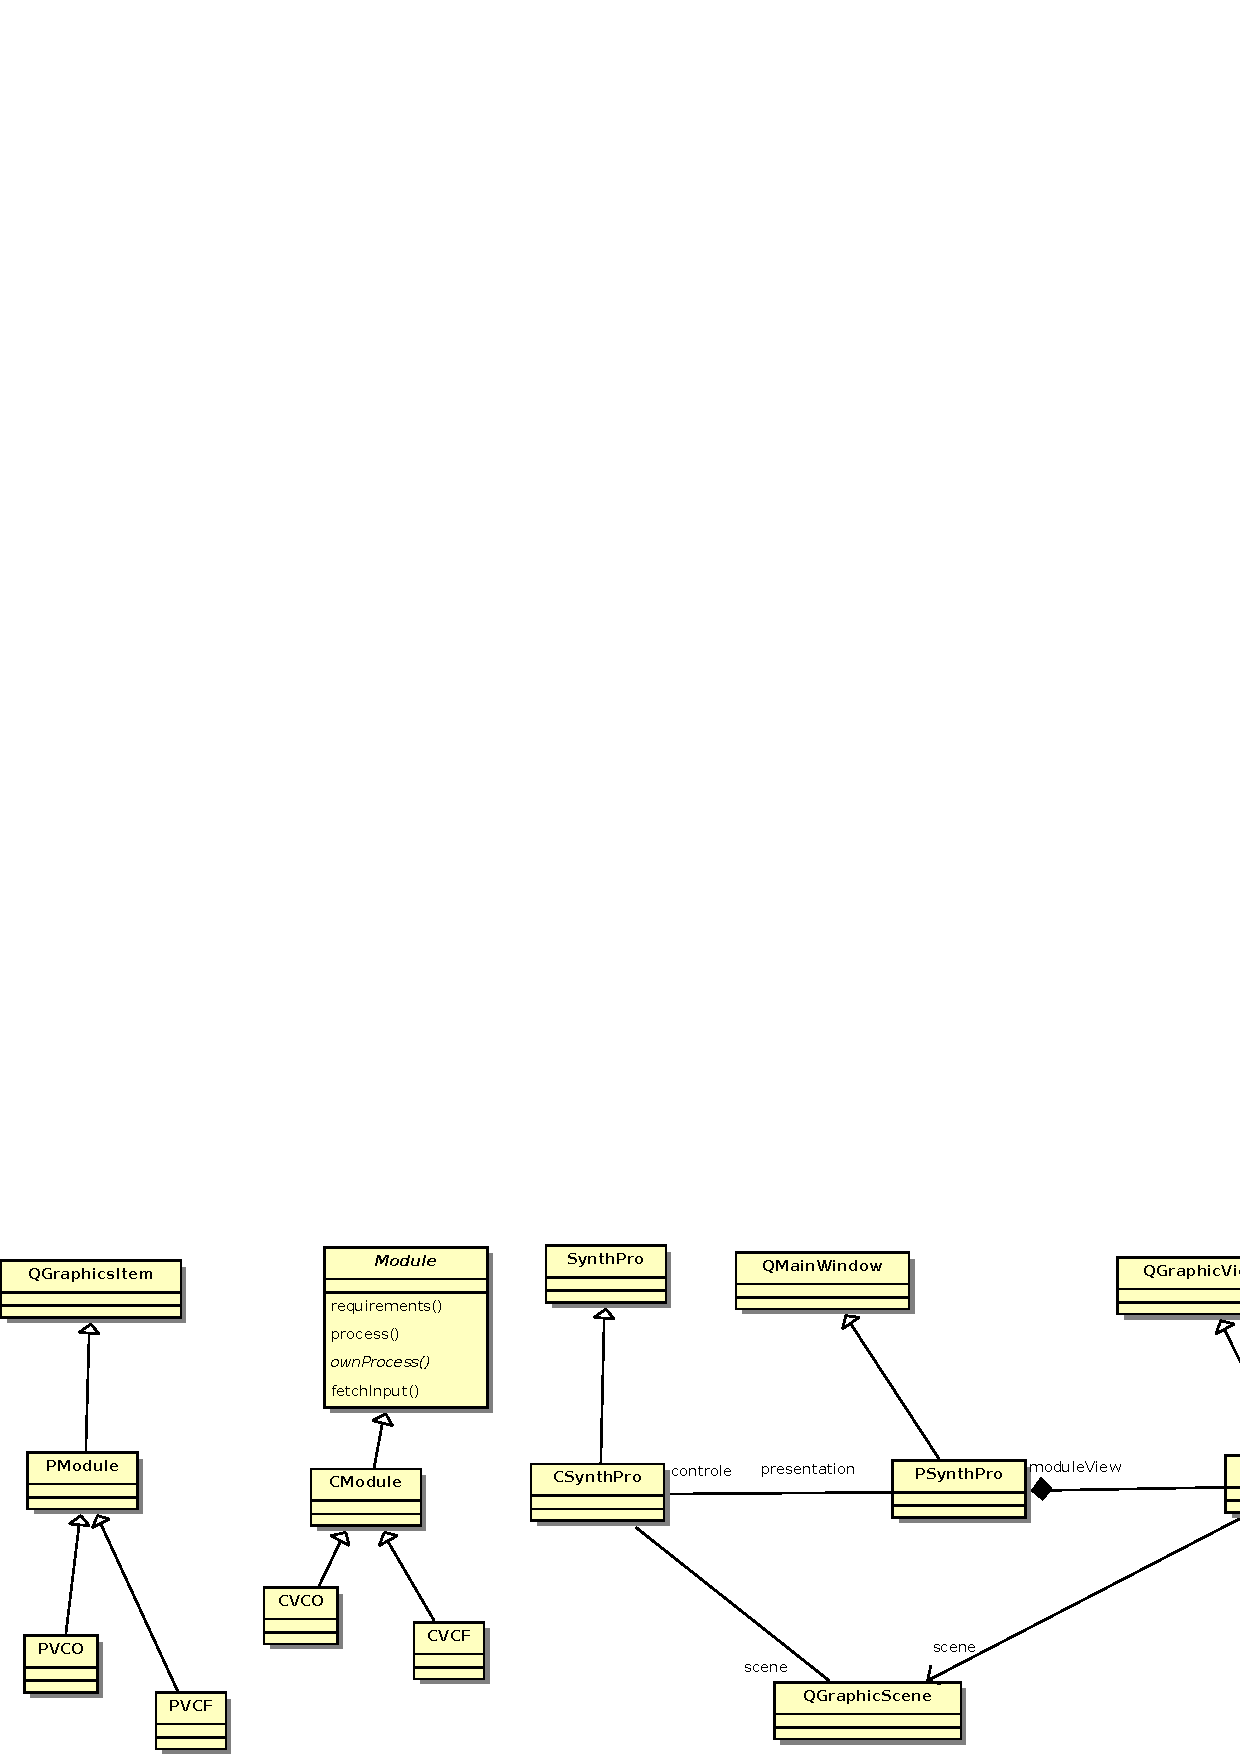
\includegraphics[width=18cm]{../img/pac.pdf}

\section{Conception PSM}
\subsection{Language et plateforme : Qt/C++}
\subsubsection{Les motivation de ce choix}
\subsubsection{Les conséquences de ce choix}
\end{document}
